\documentclass{article}
\usepackage{fullpage}

%load needed packages
\usepackage{graphicx}
\usepackage{array}
\usepackage{booktabs}
\usepackage[utf8]{inputenc}
\usepackage[T1]{fontenc}

\usepackage[spanish]{babel} % Paquete para el idioma español
\usepackage{float}  % Necesario para [H]
\usepackage{listings}
\usepackage{xcolor}
\usepackage{url}
\usepackage{tcolorbox}
\usepackage{fancybox} % Paquete para añadir sombras
\usepackage{subcaption}
\definecolor{codegreen}{HTML}{5AB2FF}
\definecolor{morado}{HTML}{AD88C6}
\definecolor{BG}{HTML}{EEEEEE}
\definecolor{azul}{HTML}{4D869C}
\definecolor{sqlblue}{HTML}{FF8C00} % Color para las palabras clave SQL

% Estilo para DDL
\lstdefinestyle{ddlstyle}{
	language=SQL,
	backgroundcolor=\color{BG},
	commentstyle=\color{codegreen},
	basicstyle=\ttfamily\small,
	keywordstyle=\color{azul},
	stringstyle=\color{morado},
	showstringspaces=false,
	breaklines=true,
	frame=shadowbox,
	numbers=left,
	numberstyle=\tiny\color{gray},
	captionpos=b,
}

% Estilo para SQL
\lstdefinestyle{sqlstyle}{
	language=SQL,
	backgroundcolor=\color{BG},
	commentstyle=\color{codegreen},
	basicstyle=\ttfamily\small,
	keywordstyle=\color{sqlblue}, % Color diferente para palabras clave SQL
	stringstyle=\color{morado},
	showstringspaces=false,
	breaklines=true,
	frame=shadowbox,
	numbers=left,
	numberstyle=\tiny\color{gray},
	captionpos=b,
}


\begin{document}



% Portada
\begin{titlepage}
	\centering
	\vspace*{3cm}
	
	% Título destacado
	{\Huge \textbf{Clinical data: deep learning approaches}\\[0.5cm]}
	
	% Espacio y logotipo (si lo tienes, por ejemplo el logo de tu universidad)
	\vspace{2cm}
	
\includegraphics[width=0.3\textwidth]{images/uma_logo.jpg}\\[1cm]
	
	% Nombre del autor
	{\LARGE \textbf{Alejandro Silva Rodríguez}\\[0.5cm]}
	{\LARGE \textbf{Marta Cuevas Rodríguez}\\[0.5cm]}
	{\large \textit{Almacenes De Datos}\\
		Universidad de Málaga\\
		}
	
	\vfill
	
	% Fecha en la parte inferior de la página
	{\large Septiembre 2024}
\end{titlepage}

% indice
\tableofcontents

\newpage
\section{Introducción}
\label{sec:introduccion}

El auge de los datos digitales en la atención médica ha conducido a un aumento en la investigación médica impulsada por datos, basada en el aprendizaje automático. En los últimos años, el aprendizaje profundo, como una técnica poderosa para el análisis de grandes datos, ha adquirido una posición central en el ámbito del aprendizaje automático debido a sus grandes ventajas en la representación de características y reconocimiento de patrones.

Los tipos de datos utilizados en este campo son diversos e incluyen datos estructurados, como registros electrónicos de salud y datos demográficos, así como datos no estructurados, como notas clínicas, imágenes médicas y secuencias genéticas. Estos datos son analizados mediante modelos de aprendizaje profundo, como redes neuronales convolucionales (CNN) para imágenes, redes neuronales recurrentes (RNN) para datos secuenciales, y modelos de atención que permiten una mejor interpretación de las relaciones entre diferentes tipos de datos. La capacidad de estos modelos para aprender de grandes volúmenes de datos ha permitido avances significativos en la predicción de enfermedades, personalización de tratamientos y optimización de la atención al paciente\cite{8787233} .




\section{Definición y Relevancia}
\subsection{¿Qué es el Deep Learning?}

Deep learning es una rama del aprendizaje automático que emplea arquitecturas de redes neuronales profundas para modelar y aprender representaciones complejas de datos. Estas arquitecturas están compuestas por múltiples capas de procesamiento, lo que permite que el sistema capture características jerárquicas y abstractas de los datos de entrada. \cite{lecun2015deep}

Los avances en deep learning han impulsado mejoras significativas en diversas áreas, como el reconocimiento de voz, la detección de objetos y la genómica, contribuyendo a la obtención de resultados de vanguardia en estas disciplinas. Utilizando el algoritmo de retropropagación, deep learning optimiza los parámetros internos del modelo, facilitando la transformación de la representación de los datos a través de las distintas capas de la red.

En particular, las redes neuronales convolucionales (CNN) han demostrado un rendimiento excepcional en tareas relacionadas con imágenes y videos, mientras que las redes neuronales recurrentes (RNN) son adecuadas para el procesamiento de datos secuenciales, como el texto y el habla. Estos enfoques han llevado a la creación de sistemas más robustos y precisos en el análisis y la interpretación de grandes volúmenes de datos.
\cite{10.1145/3234150}


\subsection{Relación con los Almacenes de Datos}

El uso de un data warehouse es fundamental en el contexto de deep learning y en la gestión de datos clínicos, ya que facilita la integración, organización y consolidación de grandes volúmenes de información provenientes de diversas fuentes. Estas fuentes pueden incluir historiales médicos, registros de laboratorio, datos de ensayos clínicos, entre otros. La estructura de un data warehouse está optimizada para la consulta de datos de forma eficiente, proporcionando un acceso rápido a información coherente y de alta calidad.

Al centralizar la información en un solo repositorio, los data warehouses no solo mejoran la eficiencia de los procesos analíticos, sino que también permiten a los investigadores y profesionales de la salud identificar patrones, tendencias y correlaciones en los datos clínicos. Esta capacidad de análisis es crucial para la toma de decisiones informadas en el ámbito de la medicina, donde cada decisión puede tener un impacto significativo en la salud del paciente. Por ejemplo, mediante el análisis de los datos almacenados en un data warehouse, es posible predecir complicaciones en pacientes de riesgo, optimizar tratamientos o incluso identificar nuevos enfoques terapéuticos basados en patrones ocultos en los datos.

El data warehouse se convierte en una herramienta indispensable para la mejora de la atención sanitaria y el avance de la investigación clínica, ya que permite integrar y analizar datos heterogéneos de manera eficiente. Además, la integración de técnicas de deep learning con data warehouses habilita aplicaciones avanzadas de aprendizaje automático en el contexto clínico. Los modelos de deep learning entrenados con datos de alta calidad pueden ayudar en la clasificación de enfermedades, la predicción de diagnósticos y la personalización de tratamientos, contribuyendo así a un enfoque más preciso y personalizado de la atención médica. \cite{hamoud2018clinical}

\section{Estado del Arte en Deep Learning para Datos Clínicos}
\label{sec:estado_del_arte}

En los últimos años, el deep learning ha experimentado un crecimiento significativo en el ámbito de la salud, especialmente en el análisis de datos clínicos. Las capacidades de los modelos de deep learning han mejorado sustancialmente con la disponibilidad de datos clínicos en gran escala y el desarrollo de infraestructuras avanzadas para el procesamiento de estos datos. En esta sección, se revisarán las tecnologías, frameworks y metodologías actuales, destacando los modelos más relevantes en el análisis de datos clínicos, como las redes neuronales convolucionales (CNNs), redes neuronales recurrentes (RNNs), y transformers. Además, se analizarán los avances recientes en la integración de almacenes de datos clínicos que facilitan el uso de deep learning en el ámbito médico.

\subsection{Tecnologías y Frameworks Actuales}

Las tecnologías de deep learning han sido impulsadas por el desarrollo de frameworks robustos, como \textit{TensorFlow} y \textit{PyTorch}, que permiten la creación, entrenamiento y despliegue de modelos de redes neuronales de manera eficiente. Estos frameworks han sido fundamentales para el análisis de grandes volúmenes de datos médicos, posibilitando el entrenamiento de modelos complejos en GPU y facilitando su implementación en plataformas clínicas. La integración de estos frameworks en entornos de investigación clínica ha permitido acelerar el desarrollo de modelos predictivos y de diagnóstico automatizado en tiempo real \cite{abadi2016tensorflow, paszke2019pytorch}.

\subsection{Modelos Clave en Deep Learning para Datos Clínicos}

El análisis de datos clínicos se ha beneficiado en gran medida de la implementación de varios tipos de modelos de deep learning que aprovechan la estructura única de estos datos. A continuación, se describen algunos de los modelos más utilizados y sus aplicaciones en el ámbito clínico.

\subsubsection{Redes Neuronales Convolucionales (CNNs)}

Las CNNs son ampliamente utilizadas en el análisis de datos de imágenes médicas, como resonancias magnéticas, tomografías y radiografías. Su capacidad para extraer y procesar características espaciales ha demostrado ser altamente efectiva en tareas de detección de enfermedades, segmentación de órganos y clasificación de imágenes. Un avance notable en este campo es el uso de redes convolucionales profundas, que permiten mejorar la precisión de diagnóstico al identificar patrones complejos en los datos visuales \cite{litjens2017survey}.

\subsubsection{Redes Neuronales Recurrentes (RNNs)}

Las RNNs y sus variantes, como LSTM (Long Short-Term Memory) y GRU (Gated Recurrent Unit), son ampliamente aplicadas en el análisis de datos secuenciales en el ámbito clínico, como el monitoreo de signos vitales o la evolución de los síntomas de un paciente a lo largo del tiempo. Estas redes permiten capturar dependencias temporales en los datos, lo cual es esencial para tareas como la predicción de eventos adversos, progresión de enfermedades y análisis de series temporales de datos clínicos \cite{choi2016doctor}.

\subsubsection{Transformers}

Más recientemente, los modelos basados en transformers han ganado popularidad debido a su eficacia en el análisis de datos secuenciales y no estructurados. Los transformers, como BERT y sus variantes, han demostrado ser altamente efectivos en el procesamiento de texto clínico, como en el análisis de notas médicas y registros de pacientes. Estos modelos son capaces de capturar relaciones contextuales complejas y han sido empleados en tareas de extracción de información clínica, codificación automática y generación de informes médicos \cite{devlin2018bert, li2020behrt}.

\subsection{Avances Recientes en Almacenes de Datos Clínicos para Deep Learning}

La consolidación y accesibilidad de grandes volúmenes de datos clínicos en almacenes de datos ha sido esencial para el desarrollo de modelos de deep learning en este campo. Un almacén de datos clínicos integra información de múltiples fuentes, incluyendo registros electrónicos de salud (EHRs), bases de datos de imágenes médicas y datos genómicos, permitiendo que los modelos de deep learning trabajen con una visión integral de la salud del paciente. Los recientes avances en la organización, limpieza y etiquetado de estos datos han mejorado la calidad y confiabilidad de los modelos, además de facilitar el análisis de relaciones entre diferentes tipos de datos clínicos \cite{miotto2018deep}.
\\

Además, el uso de almacenes de datos clínicos permite la aplicación de técnicas de aprendizaje transferido, donde los modelos entrenados en un conjunto de datos pueden ajustarse y aplicarse a otro, optimizando así el uso de los datos y reduciendo los tiempos de desarrollo. Esto es particularmente relevante en el caso de enfermedades raras, donde la cantidad de datos disponibles puede ser limitada. A medida que los sistemas de almacenes de datos clínicos se desarrollan, se espera que continúen facilitando el avance del deep learning en la medicina \cite{shickel2017deep}.

\subsection{Síntesis del Estado del Arte}

El estado del arte en deep learning aplicado a datos clínicos refleja un progreso continuo en el desarrollo de modelos robustos y precisos. La adopción de tecnologías avanzadas y frameworks especializados ha permitido mejorar el diagnóstico y la predicción de enfermedades mediante el análisis de datos clínicos complejos. La combinación de CNNs, RNNs y transformers, junto con la integración de almacenes de datos clínicos, promete impulsar aún más las capacidades del deep learning en el ámbito de la salud.
\\

\section{Metodología y Ejemplos de Uso}
\label{sec:metodologia_ejemplos}

Se implementó una aplicación web que implementa un modelo de deep learning para el diagnóstico de enfermedades dermatológicas, centrado en la clasificación de imágenes de lesiones cutáneas. A continuación, se detallan las fases del proceso:


\subsection{Entrenamiento de CNN}


\begin{enumerate}
	\item \textbf{Preparación de Datos:} El primer paso consiste en descargar el conjunto de datos desde la API de Kaggle \cite{kaggle_api}, que contiene imágenes y metadatos relevantes sobre diversas condiciones dermatológicas, concretamente el conjunto de datos Human Against Machine with 10000 (HAM10000) \cite{taha2018ham10000} que es una colección de imágenes dermatoscópicas que se utiliza para la clasificación de diferentes tipos de cáncer de piel. 
	
	Se realiza un análisis inicial de los datos para identificar el desequilibrio en las clases. En este caso, se observa que la clase de lunares ('nv') tiene una cantidad significativamente mayor de imágenes en comparación con otras clases. Para abordar este problema, se decide reducir el número de imágenes de lunares a un 40\% de su cantidad original, asegurando así un mejor equilibrio en el conjunto de datos .
	
	\item \textbf{División de Datos:} Una vez que los datos se han equilibrado, se procede a dividir el conjunto en datos de entrenamiento y de validación. Se utiliza una proporción del 80\% de los datos para el entrenamiento y el 20\% restante para la validación. Esto garantiza que el modelo sea capaz de generalizar a nuevos datos y no se limite a memorizar el conjunto de entrenamiento.
	
	\item \textbf{Generación de Datos:} Para mejorar la capacidad del modelo para generalizar, se implementan generadores de datos que aplican técnicas de aumento de imágenes, como rotaciones, escalados y cambios de brillo. Esto no solo aumenta la cantidad de datos disponibles para el entrenamiento, sino que también ayuda a simular variaciones que el modelo puede encontrar en situaciones del mundo real.
	
	\item \textbf{Entrenamiento del Modelo:} Se utilizó MobileNetV2 \cite{mobilenetv2}, un modelo preentrenado en la base de datos ImageNet, lo que permitió aprovechar características previamente aprendidas para mejorar la precisión en la clasificación de imágenes de piel. 
	
	El entrenamiento se llevó a cabo con TensorFlow \cite{abadi2016tensorflow}, donde se implementaron técnicas de Dropout y Early Stopping para mitigar el riesgo de sobreajuste. El Dropout se utilizó para desactivar aleatoriamente un porcentaje de neuronas durante el entrenamiento, promoviendo la generalización del modelo. Por otro lado, el Early Stopping supervisó la precisión en el conjunto de validación y detuvo el entrenamiento automáticamente cuando no se observaron mejoras durante un número definido de épocas. Además, se congelaron las capas iniciales de MobileNetV2, permitiendo que las capas superiores se ajustaran finamente a los datos específicos del problema. Esta estrategia resultó en un modelo eficiente y robusto para el diagnóstico de enfermedades cutáneas.
	
	\item \textbf{Evaluación y Ajuste del Modelo:} Tras el entrenamiento, se evalúa el modelo en el conjunto de validación utilizando métricas como precisión y pérdida. Además, se generan matrices de confusión para analizar el rendimiento en cada clase. Se ajustan los umbrales de decisión, particularmente para la clase de lunares, para minimizar los falsos positivos, asegurando así que el modelo sea más confiable en la identificación de esta condición crítica \cite{esteva2017dermatologist}.
\end{enumerate}

\subsection{Aplicación Web}

La aplicación web fue desarrollada utilizando el framework de Python, FastAPI, y se implementaron dos endpoints principales para la interacción con el modelo y el usuario.

\begin{itemize}
	\item \textbf{Endpoint raíz:} Este endpoint sirve los archivos estáticos que verá el usuario, incluyendo el HTML, CSS y JavaScript necesarios para abrir la cámara del dispositivo y capturar una imagen. La interfaz (Figura \ref{fig:app_interface}) permite al usuario capturar la imagen que se enviará al modelo de diagnóstico y muestra tanto las imágenes procesadas como los resultados de la predicción de enfermedades dermatológicas.
	
	\item \textbf{Endpoint de Procesamiento de Fotogramas (/video\_frame/):} Este endpoint recibe un fotograma, lo pasa por el modelo de detección de enfermedades y devuelve la respuesta con el diagnóstico. Se implementaron certificados SSL autofirmados para que la aplicación pueda acceder a la cámara del dispositivo en navegadores web, lo cual es especialmente importante para asegurar la privacidad y confidencialidad de los datos.
\end{itemize}

\begin{figure}[H]
	\centering
	\begin{subfigure}[t]{0.45\textwidth}
		\centering
		\shadowbox{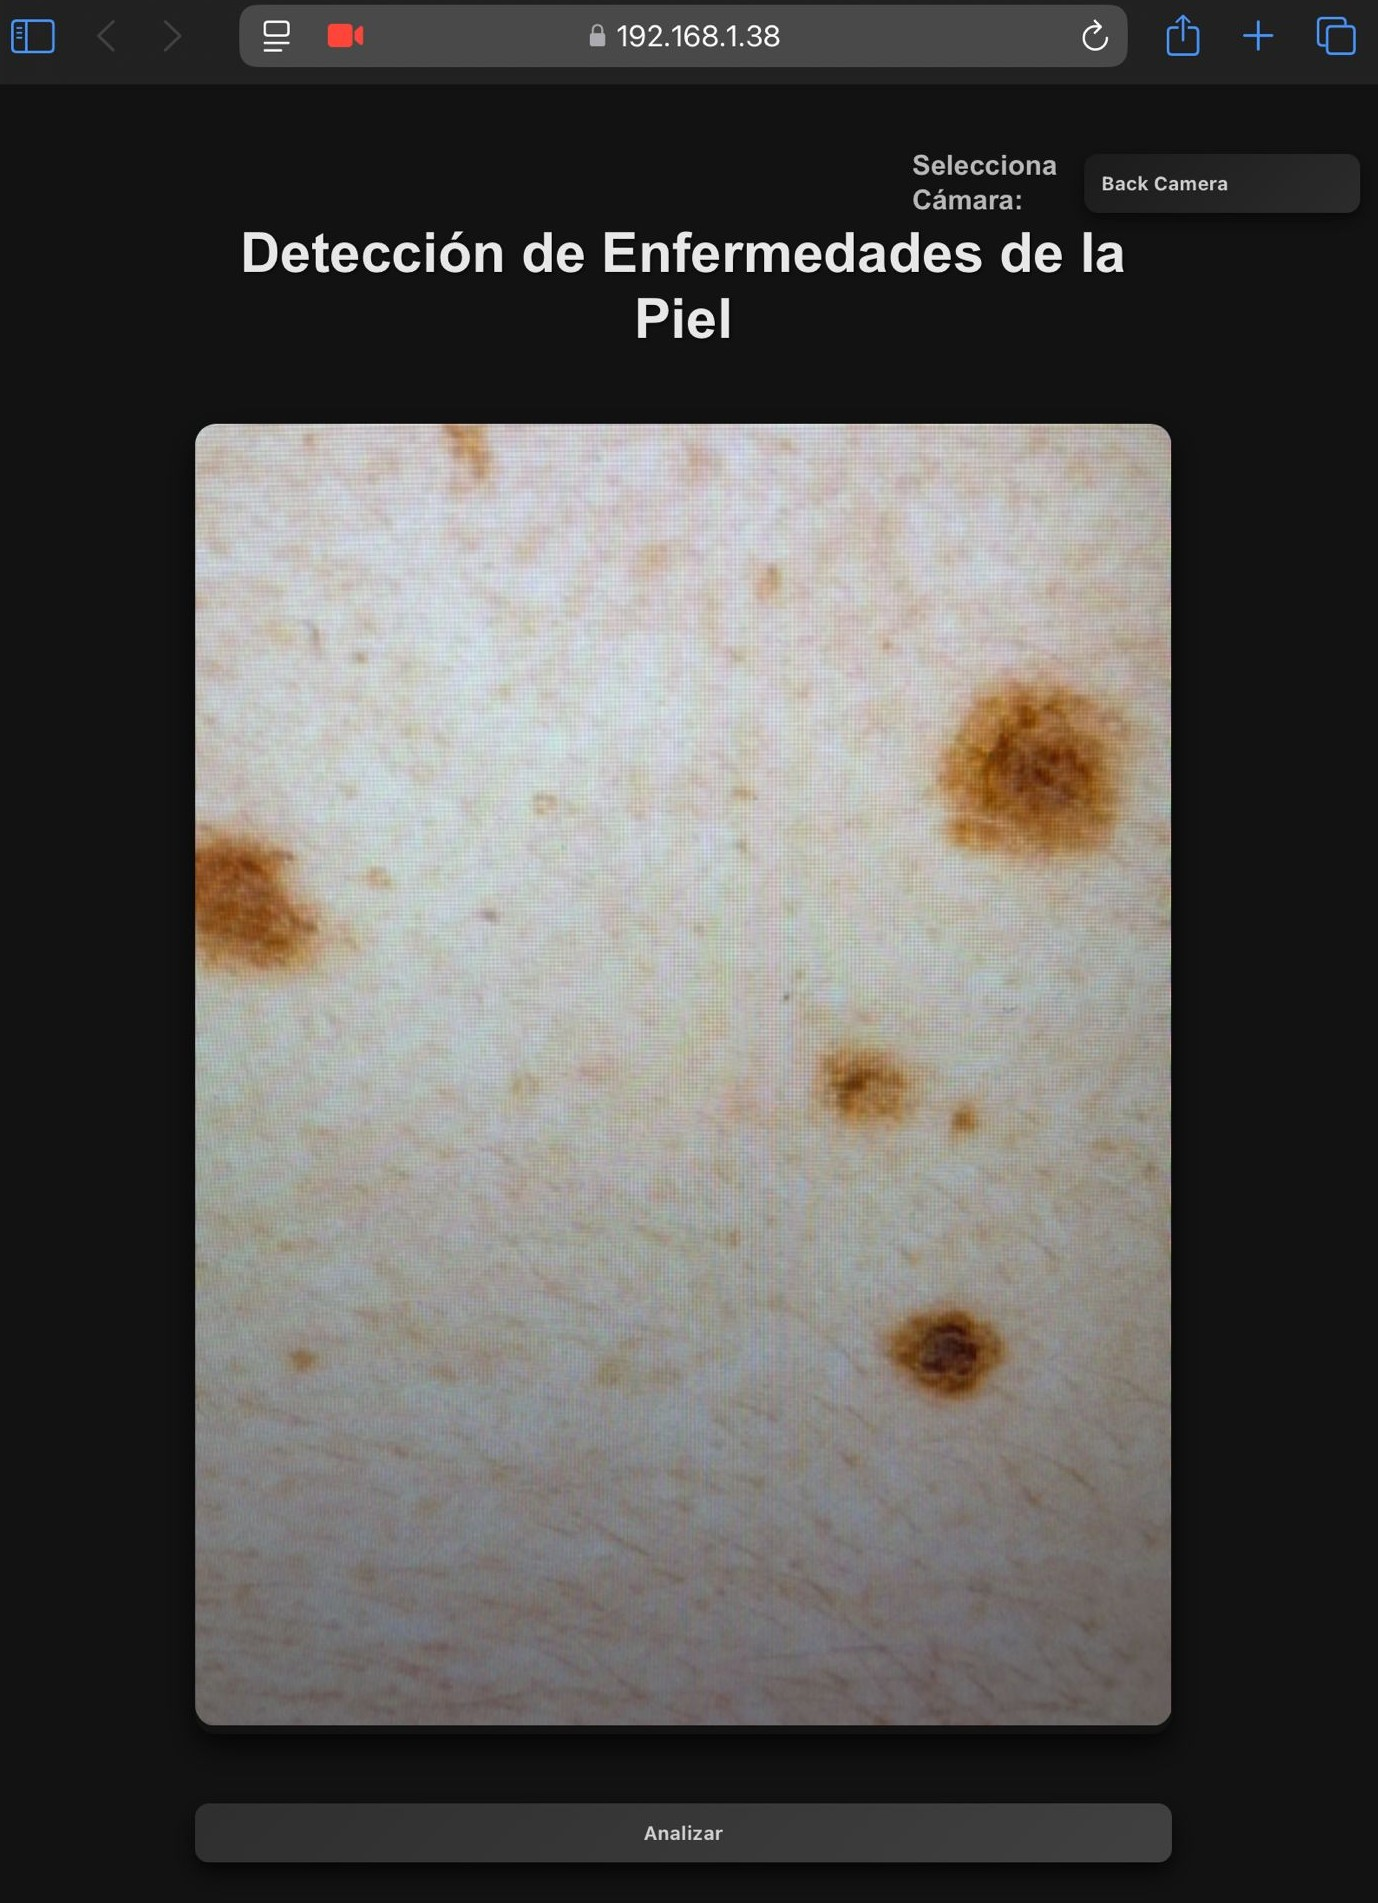
\includegraphics[width=\textwidth]{images/app1.jpeg}}
		\caption{Cámara de la app}
	\end{subfigure}%
	\hspace{0.05\textwidth}
	\begin{subfigure}[t]{0.45\textwidth}
		\centering
		\shadowbox{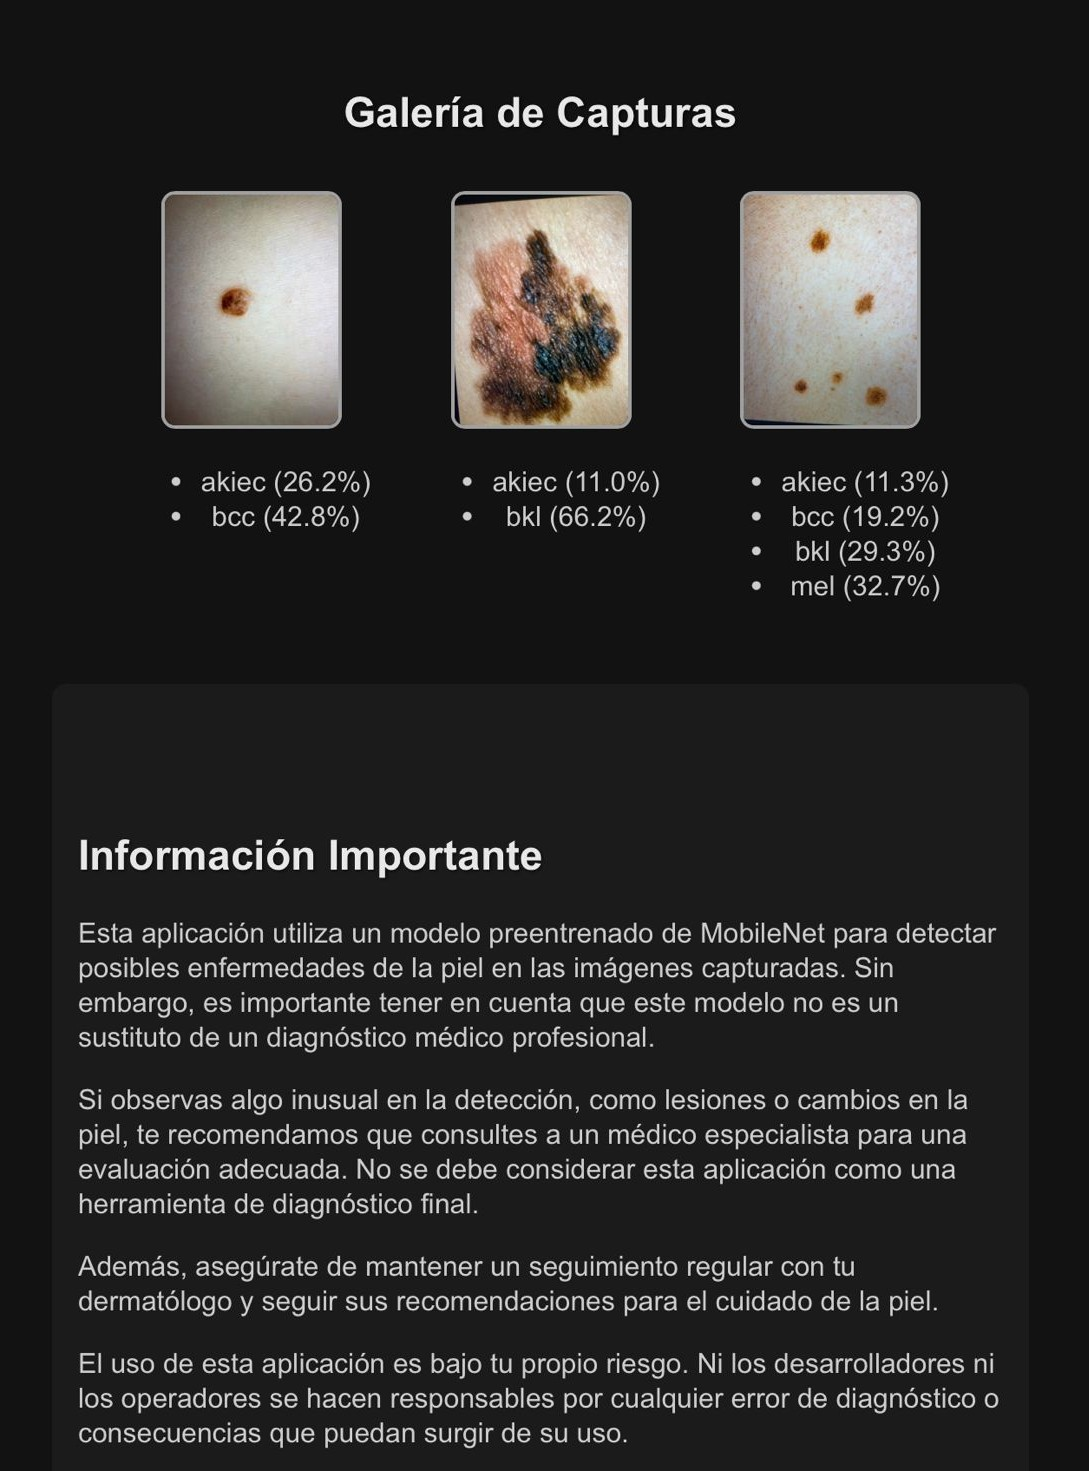
\includegraphics[width=\textwidth]{images/app2.jpeg}}
		\caption{Galería de la app}
	\end{subfigure}
	\caption{Interfaz de la aplicación: acceso a la cámara y galería}
	\label{fig:app_interface}
\end{figure}
Esta aplicación es multiplataforma gracias a su naturaleza web, permitiendo su uso en diferentes dispositivos sin necesidad de instalaciones adicionales. La implementación de FastAPI facilita el procesamiento eficiente y seguro de las imágenes, lo que permite al usuario recibir un diagnóstico casi en tiempo real en cualquier dispositivo con acceso a internet y cámara.
\section{Desafíos y Direcciones Futuras}

A pesar de los avances significativos en el uso de deep learning para datos clínicos, todavía existen desafíos clave que limitan la implementación generalizada de estas tecnologías en entornos de salud. Uno de los problemas más importantes es la calidad y disponibilidad de los datos clínicos. La variabilidad en los sistemas de registros electrónicos de salud y la falta de interoperabilidad entre diferentes plataformas dificultan la integración de datos de múltiples fuentes, lo cual es crucial para entrenar modelos robustos y generalizables \cite{johnson2016mimic}.

Otro desafío se encuentra en la interpretabilidad de los modelos de deep learning, especialmente en el ámbito clínico, donde las decisiones automatizadas deben ser justificables y comprensibles para los profesionales de la salud. El desarrollo de modelos explicables y transparentes representa una gran oportunidad para que el deep learning sea adoptado con confianza en el sector médico \cite{holzinger2017we}.

Asimismo, el área de privacidad y seguridad de los datos sigue siendo una preocupación crítica, particularmente debido a la naturaleza sensible de los datos de salud. La investigación en técnicas como el aprendizaje federado y la privacidad diferencial ofrece un camino prometedor para abordar estas cuestiones y facilitar el entrenamiento de modelos sin comprometer la privacidad de los pacientes \cite{rieke2020future}.

En el futuro, es probable que el desarrollo de herramientas que combinen múltiples tipos de datos clínicos y la aplicación de enfoques multimodales amplíen las capacidades del deep learning en el campo de la salud. Estos enfoques podrían mejorar la precisión y el alcance de los modelos, ofreciendo aplicaciones que vayan desde la detección temprana de enfermedades hasta la personalización de tratamientos.


\newpage
\section{Acceso al Repositorio}

Toda la información adicional, incluyendo el código fuente y la documentación completa de este proyecto, está disponible en el repositorio de GitHub \cite{silva2024github}.

% Incluir la bibliografía
\bibliographystyle{plain}  % Estilo de la bibliografía (por ejemplo, plain, alpha, ieee, etc.)
\bibliography{bibli}  % Nombre del archivo .bib sin la extensión

\end{document}
